% Created 2021-09-27 lun 10:53
% Intended LaTeX compiler: pdflatex
\documentclass[aspectratio=169, xcolor={usenames,svgnames,dvipsnames}]{beamer}
\usepackage[utf8]{inputenc}
\usepackage[T1]{fontenc}
\usepackage{graphicx}
\usepackage{grffile}
\usepackage{longtable}
\usepackage{wrapfig}
\usepackage{rotating}
\usepackage[normalem]{ulem}
\usepackage{amsmath}
\usepackage{textcomp}
\usepackage{amssymb}
\usepackage{capt-of}
\usepackage{hyperref}
\usepackage{color}
\usepackage{listings}
\usepackage{mathpazo}
\usepackage{gensymb}
\usepackage{amsmath}
\usepackage{diffcoeff}
\usepackage{steinmetz}
\usepackage{mathtools}
\bibliographystyle{plain}
\usepackage[emulate=units]{siunitx}
\sisetup{fraction=nice, decimalsymbol=comma, retain-unity-mantissa = false}
\newunit{\wattpeak}{Wp}
\newunit{\watthour}{Wh}
\newunit{\amperehour}{Ah}
\hypersetup{colorlinks=true, linkcolor=Blue, urlcolor=Blue}
\renewcommand{\thefootnote}{\fnsymbol{footnote}}
\newcommand{\laplace}[1]{\mathbf{#1}(\mathbf{s})}
\newcommand{\slp}{\mathbf{s}}
\newcommand{\fasor}[1]{\mathbf{#1}(\omega)}
\newcommand{\atan}{\mathrm{atan}}
\parskip=5pt
\usetheme{Boadilla}
\usecolortheme{rose}
\usefonttheme{serif}
\author{Oscar Perpiñán Lamigueiro}
\date{}
\title{Fundamentos. Circuitos de Corriente Continua.}
\subtitle{Teoría de Circuitos}
\setbeamercolor{alerted text}{fg=blue!50!black} \setbeamerfont{alerted text}{series=\bfseries}
\AtBeginSubsection[]{\begin{frame}[plain]\tableofcontents[currentsubsection,sectionstyle=show/shaded,subsectionstyle=show/shaded/hide]\end{frame}}
\AtBeginSection[]{\begin{frame}[plain]\tableofcontents[currentsection,hideallsubsections]\end{frame}}
\beamertemplatenavigationsymbolsempty
\setbeamertemplate{footline}[frame number]
\setbeamertemplate{itemize items}[triangle]
\setbeamertemplate{enumerate items}[circle]
\setbeamertemplate{section in toc}[circle]
\setbeamertemplate{subsection in toc}[circle]
\hypersetup{
 pdfauthor={Oscar Perpiñán Lamigueiro},
 pdftitle={Fundamentos. Circuitos de Corriente Continua.},
 pdfkeywords={},
 pdfsubject={},
 pdfcreator={Emacs 27.1 (Org mode 9.4.6)}, 
 pdflang={Spanish}}
\begin{document}

\maketitle

\section{Conceptos Fundamentales}
\label{sec:orgfcab559}
\subsection{Teoría de Circuitos}
\label{sec:orga9ec030}
\begin{frame}[label={sec:org9088b6f}]{}
Este curso está dedicado al \alert{análisis} de \alert{circuitos eléctricos} \alert{lineales} de \alert{parámetros concentrados}.
\end{frame}
\begin{frame}[label={sec:org33bdc2c}]{Circuito Eléctrico}
Un \alert{circuito eléctrico} es un conjunto de componentes eléctricos interconectados mediante conductores que crean un camino cerrado por el que puede circular corriente eléctrica. 

Un circuito eléctrico puede incluir:
\begin{itemize}
\item \alert{elementos activos} (generadores), que entregan potencia al circuito
\item \alert{elementos pasivos} (receptores), que consumen o almacenan la potencia que circula.
\end{itemize}
\end{frame}

\begin{frame}[label={sec:org428a06d}]{Análisis y Diseño}
El \alert{análisis} (o resolución) de un circuito eléctrico existente persigue determinar sus condiciones de funcionamiento:
\begin{enumerate}
\item Definir las ecuaciones correspondientes al circuito,
\item Obtener los valores de determinadas variables importantes a partir de dichas ecuaciones.
\end{enumerate}

El \alert{diseño} (o síntesis) de un circuito eléctrico tiene como objetivo definir el circuito eléctrico, es decir, determinar los componentes necesarios y su interconexión, para obtener unas condiciones de funcionamiento.
\end{frame}
\begin{frame}[label={sec:orgedcb252}]{Sistemas lineales}
Todos los circuitos eléctricos que se estudian en este curso se comportan como \alert{sistemas lineales}: 

\begin{itemize}
\item \(f(x + y) = f(x) + f(y)\)

La respuesta \(f\) a la suma de dos entradas \(x\) e \(y\) es igual a la suma de la respuesta individual a cada una de las entradas
\item \(f(k \cdot x) = k \cdot f(x)\)

La respuesta a una entrada que está multiplicada por un factor de escala \(k\) es igual a multiplicar por este factor a la respuesta a la entrada.
\end{itemize}
\end{frame}

\begin{frame}[label={sec:orgd4a9815}]{La linealidad es una aproximación de la realidad}
\begin{itemize}
\item Estas propiedades simplifican el tratamiento de los circuitos, y \alert{permiten aplicar técnicas de resolución de ecuaciones lineales}.
\item La linealidad es una \alert{aproximación de la realidad} que no puede aplicarse de manera indiscriminada a cualquier componente y en cualquier condición.
\item En particular, los \alert{dispositivos electrónicos} como diodos o transistores tienen un \alert{comportamiento} marcadamente \alert{no lineal}, de forma que los circuitos que los contienen no pueden analizarse directamente con las técnicas que aquí se exponen sin realizar previamente aproximaciones de su funcionamiento.
\end{itemize}
\end{frame}

\begin{frame}[label={sec:orgdb50c6c}]{Parámetros concentrados}
\begin{itemize}
\item Los circuitos eléctricos reales ocupan espacio, las máquinas generadoras y los receptores tienen grandes dimensiones, y los cables conductores se extienden a lo largo de longitudes variopintas.
\item Sin embargo, el análisis de circuitos no toma en consideración las propiedades espaciales de los circuitos ni de sus componentes, sino que los confina a elementos puntuales con un modelo de \alert{parámetros concentrados}.
\item Por ejemplo, un conductor real de \(\SI{100}{\meter}\) se representará habitualmente como un conductor ideal con una resistencia en su punto medio.
\end{itemize}
\end{frame}
\begin{frame}[label={sec:org65c2133}]{Simplificación de las ecuaciones de Maxwell}
\begin{itemize}
\item Este tratamiento es una simplificación de las ecuaciones del electromagnetismo de Maxwell
\item Es aplicable únicamente cuando las dimensiones del circuito real son inferiores a la longitud de onda de la señal que circula por el circuito.
\item Por ejemplo:
\begin{itemize}
\item A la frecuencia de \(\SI{50}{\hertz}\), habitual en sistemas eléctricos industriales, la longitud de onda de la señal es de \(\SI{6000}{\kilo\meter}\).
\item A la frecuencia de \(\SI{2.6}{\giga\hertz}\), característica de la telefonía 4G, la longitud de onda se reduce a \(\SI{11.5}{\centi\meter}\).
\end{itemize}
\end{itemize}
\end{frame}


\subsection{Variables}
\label{sec:org6a50306}
\begin{frame}[label={sec:org4e59a29}]{Tensión Eléctrica}
El \alert{potencial eléctrico en un punto}, \(v(t)\),  es la energía potencial que tiene una carga unitaria en ese punto debida al campo eléctrico. 

\begin{center}
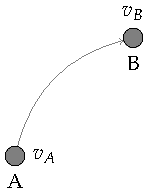
\includegraphics[height=0.3\textheight]{figs/tension_puntos.pdf}
\end{center}

La \alert{tensión o diferencia de potencial entre dos puntos} A y B, \(u_{AB}(t)\), es el trabajo realizado por el campo eléctrico al desplazar una carga unitaria entre esos puntos. 

\begin{equation*}
  u_{AB}(t) = v_A(t) - v_B(t) = \frac{dW_{e}}{dq}
\end{equation*}

La \alert{unidad} de la tensión eléctrica es el \alert{voltio} (V).
\end{frame}

\begin{frame}[label={sec:orgdbaccc6}]{La trayectoria no importa}
Dado que el campo eléctrico es \alert{conservativo}, la diferencia de potencial entre A y B \alert{no depende de la trayectoria} seguida para realizar el desplazamiento, sino únicamente del potencial existente en cada uno de los puntos. 

\begin{center}
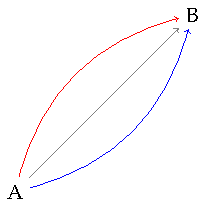
\includegraphics[height=0.6\textheight]{figs/diagrama_tension.pdf}
\end{center}
\end{frame}

\begin{frame}[label={sec:org2aba407}]{El signo depende del sentido}
Aunque la trayectoria no sea relevante para el cálculo de la tensión, siempre hay que tener en cuenta el \alert{sentido del desplazamiento}. 

\begin{center}
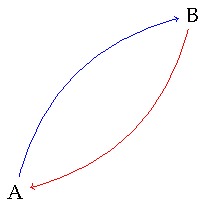
\includegraphics[height=0.4\textheight]{figs/sentido_tension.pdf}
\end{center}

Así, si el movimiento se produce desde B hasta A obtenemos el signo contrario al anterior resultado:

\begin{equation*}
  u_{BA} = v_B - v_A = - u_{AB} 
\end{equation*}
\end{frame}

\begin{frame}[label={sec:org76b13a1}]{Corriente Eléctrica}
Se define la \alert{intensidad de la corriente eléctrica} como la variación de la carga \(q(t)\) que atraviesa la sección transversal de un conductor por unidad de tiempo:

\begin{equation*}
  i(t)=\frac{dq(t)}{dt}
\end{equation*}

\begin{center}
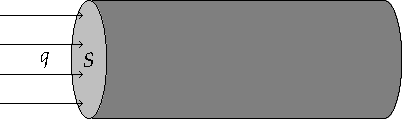
\includegraphics[height=0.2\textheight]{figs/seccion_conductor.pdf}
\end{center}

La corriente eléctrica se produce por el \alert{movimiento de los electrones libres} que fluyen por el conductor. Sin embargo, por razones históricas, el \alert{convenio} que se se emplea considera como sentido de la corriente el debido al \alert{movimiento de las cargas positivas}.

La \alert{unidad} de la corriente es el \alert{amperio} (A).
\end{frame}

\begin{frame}[label={sec:org1dc7981}]{Potencia Eléctrica}
La \alert{potencia eléctrica} es la variación del trabajo del campo eléctrico por unidad de tiempo:

\begin{equation*}
  p(t)=\frac{dW_{e}}{dt}
\end{equation*}

Esta definición genérica puede relacionarse con las anteriores variables:

\begin{align*}
  p(t) &= \frac{dW_e}{dq} \cdot \frac{dq(t)}{dt}\\
       &= v(t)\cdot i(t)
\end{align*}

La \alert{unidad} de la potencia eléctrica es el \alert{vatio} (W).
\end{frame}

\begin{frame}[label={sec:org7ab9240}]{Signo de la potencia eléctrica}
Para determinar el \alert{signo de la potencia eléctrica} hay que tener en consideración los signos de las variables de las que depende, la tensión y la corriente. 
\begin{itemize}
\item Cuando las flechas de ambas variables tienen el \alert{mismo sentido} la potencia eléctrica es \alert{positiva}
\item Cuando las flechas tienen \alert{sentidos opuestos} la potencia eléctrica es \alert{negativa}.
\end{itemize}

\begin{center}
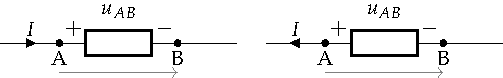
\includegraphics[height=0.2\textheight]{figs/signo_potencia.pdf}
\end{center}
\end{frame}

\begin{frame}[label={sec:org088bb90}]{Receptores y Generadores}
Es habitual \alert{interpretar} este resultado en términos de potencia absorbida o potencia entregada. 
\begin{itemize}
\item Un \alert{circuito receptor absorbe potencia} y la corriente \emph{entra} por el terminal de mayor potencial,
\item Un \alert{circuito generador entrega potencia} y la corriente \emph{sale} por el terminal de mayor potencial.
\end{itemize}

\begin{center}
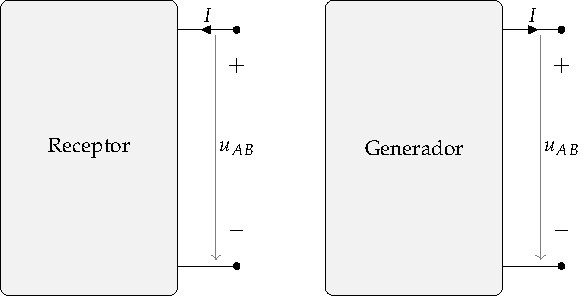
\includegraphics[height=0.5\textheight]{figs/receptor_generador.pdf}
\end{center}
\end{frame}

\begin{frame}[label={sec:org0b4b504}]{Potencia y Energía}
\begin{description}
\item[{Energía}] es la capacidad para realizar un trabajo.

Unidades Wh, kWh

1 kWh = 3.6 MJ

\item[{Potencia}] es la cantidad de trabajo efectuado \emph{por unidad de
tiempo}.

Unidades W, kW
\end{description}
\end{frame}

\begin{frame}[label={sec:org6dcb3e4}]{Rendimiento/Eficiencia}
Cuadripolo (entrada/salida)
\begin{equation*}
  \eta = \frac{P_{salida}}{P_{entrada}}
\end{equation*}

Receptor
\begin{equation*}
  \eta_m = \frac{P_{util}}{P_{absorbida}}
\end{equation*}

Generador
\begin{equation*}
  \eta_g = \frac{P_{entregada}}{P_{producida}}
\end{equation*}

Cualquier máquina tiene pérdidas:

\begin{equation*}
  \boxed{\eta < 1}
\end{equation*}
\end{frame}

\begin{frame}[label={sec:org3885e6d}]{Corriente Continua y Corriente Alterna}
\begin{itemize}
\item Corriente Continua (\(\frac{d}{dt} = 0\))
\end{itemize}
\begin{center}
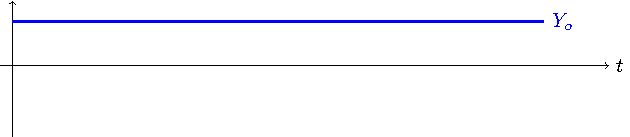
\includegraphics[height=0.25\textheight]{figs/continua.pdf}
\end{center}

\begin{itemize}
\item Corriente Alterna (\(\frac{d}{dt} \neq 0\))
\end{itemize}
\begin{center}
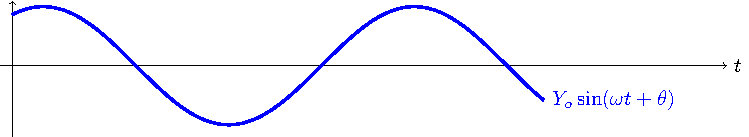
\includegraphics[height=0.25\textheight]{figs/sin.pdf}
\end{center}
\end{frame}

\section{Elementos circuitales}
\label{sec:orgadb0aec}

\subsection{Elementos Pasivos}
\label{sec:org560a716}
\begin{frame}[label={sec:org37c77ef}]{Resistencia}
\begin{itemize}
\item \alert{Ley de Ohm}: una resistencia provoca una \alert{diferencia de potencial} entre sus terminales \alert{directamente proporcional} a su corriente: \alert{resistencia} (Ohmios, [\(\Omega\)])
\end{itemize}
\[
u(t) = R \cdot i(t)
\]
\begin{itemize}
\item \alert{Criterio de Signos}: la tensión es positiva en el terminal por el que entra la corriente (las flechas de tensión y corriente tienen el mismo sentido).
\end{itemize}
\begin{columns}
\begin{column}{0.5\columnwidth}
\begin{center}
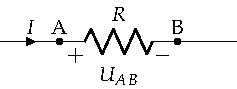
\includegraphics[height=0.2\textheight]{figs/Resistencia.pdf}
\end{center}
\end{column}
\begin{column}{0.5\columnwidth}
\begin{center}
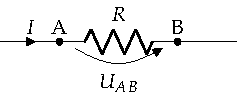
\includegraphics[height=0.2\textheight]{figs/Resistencia_Flecha.pdf}
\end{center}
\end{column}
\end{columns}
\end{frame}

\begin{frame}[label={sec:org962c5fc}]{Resistividad}
\begin{itemize}
\item El valor de la resistencia depende de la \alert{resistividad del material} (\(\rho\)), de la \alert{sección} (\(S\)), y de la
longitud (\(l\)):
\end{itemize}
\begin{equation*}
  R = \rho \cdot \frac{l}{S}
\end{equation*}

\begin{itemize}
\item La \alert{sección} se expresa en \(\si{\milli\meter\squared}\).

\item La \alert{resistividad} depende del material conductor y de la temperatura ambiente:

\begin{itemize}
\item Cobre a 20ºC: \(\SI{17.24}{\milli\ohm\milli\meter\squared\per\meter}\).
\end{itemize}
\end{itemize}
\end{frame}

\begin{frame}[label={sec:org2fe5448}]{Cortocircuito y Circuito Abierto}
\begin{itemize}
\item Cortocircuito: resistencia nula (tensión nula)
\end{itemize}

\begin{center}
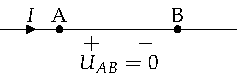
\includegraphics[height=0.2\textheight]{figs/Cortocircuito.pdf}
\end{center}

\begin{itemize}
\item Circuito abierto: resistencia infinita (corriente nula).
\end{itemize}

\begin{center}
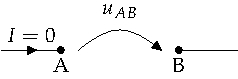
\includegraphics[height=0.2\textheight]{figs/CircuitoAbierto.pdf}
\end{center}
\end{frame}

\begin{frame}[label={sec:org0961e30}]{Ley de Joule}
\begin{center}
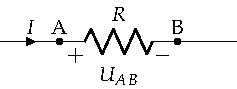
\includegraphics[height=0.2\textheight]{figs/Resistencia.pdf}
\end{center}

\begin{itemize}
\item \alert{Ley de Joule}: una resistencia disipa energía eléctrica produciendo \alert{calor}.
\end{itemize}
\[
p(t)=R\cdot i^{2}(t)
\]
\end{frame}


\begin{frame}[label={sec:orgc0cba7b}]{Bobina o inductancia}
\begin{center}
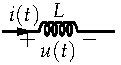
\includegraphics[height=0.2\textheight]{figs/Bobina.pdf}
\end{center}

\begin{itemize}
\item Cuando una corriente oscilante atraviesa un conductor arrollado alrededor de un núcleo, se produce una \alert{tensión inducida que se opone a esta corriente} (ley de Faraday y Lenz)

\item La tensión en sus terminales es directamente proporcional al cambio de la corriente: coeficiente de autoinducción o \alert{inductancia} (Henrios [H]).
\end{itemize}

\[
u_L(t)=L\cdot\frac{di(t)}{dt}
\]
\end{frame}

\begin{frame}[label={sec:org9944ee6}]{Bobina o inductancia}
\begin{center}
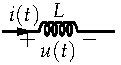
\includegraphics[height=0.2\textheight]{figs/Bobina.pdf}
\end{center}

\begin{itemize}
\item Almacena \alert{energía magnética}.
\end{itemize}

\[
  E_L(t) = \int_{-\infty}^t u(\tau) \cdot i(\tau) d\tau = \frac{1}{2} \cdot L \cdot i^2(t)
\]
\begin{itemize}
\item En circuitos de corriente continua es un cortocircuito.
\end{itemize}

\begin{equation*}
  \frac{di(t)}{dt} = 0 \Rightarrow U_L = 0
\end{equation*}
\end{frame}

\begin{frame}[label={sec:org3ef274c}]{Condensador}
\begin{center}
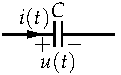
\includegraphics[height=0.2\textheight]{figs/Condensador.pdf}
\end{center}

\begin{itemize}
\item Un \alert{condensador} está formado por dos placas metálicas separadas por una capa dieléctrica. Al aplicar tensión se produce una \alert{separación de cargas opuestas} que se \alert{acumulan} en cada placa.

\item La \alert{carga acumulada} en un instante es \alert{proporcional} a la \alert{diferencia de potencial} en ese instante: \alert{capacidad} (Faradios [F]).
\end{itemize}

\[
q(t) = C \cdot u(t)
\]

\begin{itemize}
\item En el proceso de carga se produce una corriente eléctrica entre las dos placas.
\end{itemize}
\[
i_C(t)=\frac{dq(t)}{d(t)}=C\frac{du(t)}{dt}
\]
\end{frame}


\begin{frame}[label={sec:orgf3538e7}]{Condensador}
\begin{center}
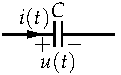
\includegraphics[height=0.2\textheight]{figs/Condensador.pdf}
\end{center}

\begin{itemize}
\item Un condensador almacena \alert{energía eléctrica}
\end{itemize}

\[
  E_c(t) = \int_{-\infty}^t u(\tau) \cdot i(\tau) d\tau = \frac{1}{2} \cdot C \cdot u^2(t)
\]

\begin{itemize}
\item En un circuito de corriente continua se comporta como un circuito abierto.
\end{itemize}

\begin{equation*}
  \frac{du(t)}{dt} = 0 \Rightarrow I_c = 0
\end{equation*}
\end{frame}

\subsection{Elementos Activos}
\label{sec:orgf387284}

\begin{frame}[label={sec:orgd6db9cf}]{Generadores de Tensión y Corriente}
\begin{columns}
\begin{column}{0.5\columnwidth}
\begin{center}
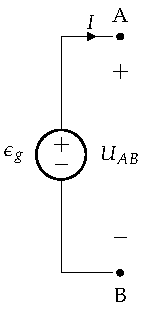
\includegraphics[height=0.5\textheight]{figs/FuenteTensionIdealDC.pdf}
\end{center}
Un \alert{generador de tensión ideal} impone la tensión a la salida (\emph{la corriente depende del circuito}). Se caracteriza por su \alert{fuerza electromotriz} (voltios [V]).
\end{column}

\begin{column}{0.5\columnwidth}
\begin{center}
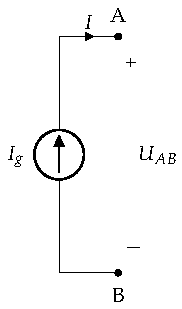
\includegraphics[height=0.5\textheight]{figs/FuenteCorrienteIdeal.pdf}
\end{center}
Un \alert{generador de corriente ideal} impone la corriente a la salida (\emph{la tensión depende del circuito}). Se caracteriza por su corriente de generador.
\end{column}
\end{columns}
\end{frame}

\begin{frame}[label={sec:org31dd1b7}]{Generador Real}
Los generadores reales tienen pérdidas que se modelan con una resistencia en \alert{serie} (generador de tensión) o en \alert{paralelo} (generador de corriente)

\begin{columns}
\begin{column}{0.5\columnwidth}
\begin{center}
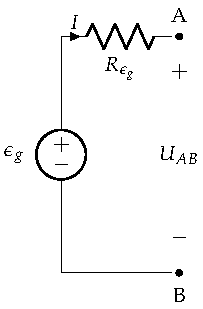
\includegraphics[height=0.7\textheight]{figs/FuenteTensionRealDC.pdf}
\end{center}
\end{column}
\begin{column}{0.5\columnwidth}
\begin{center}
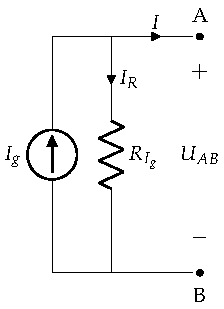
\includegraphics[height=0.7\textheight]{figs/FuenteCorrienteRealDC.pdf}
\end{center}
\end{column}
\end{columns}
\end{frame}


\section{Leyes de Kirchhoff}
\label{sec:orgc7fda1a}

\subsection{Definiciones}
\label{sec:org2568ba4}
\begin{frame}[label={sec:org68d3153}]{Nudo, rama, malla}
\begin{description}
\item[{Nudo}] unión de \alert{3} o más conductores.
\item[{Rama}] elementos conectados entre dos nudos consecutivos.
\item[{Lazo}] conjunto de ramas que forman un camino cerrado.
\item[{Malla}] lazo que no contiene ningún otro en su interior.
\end{description}

\begin{center}
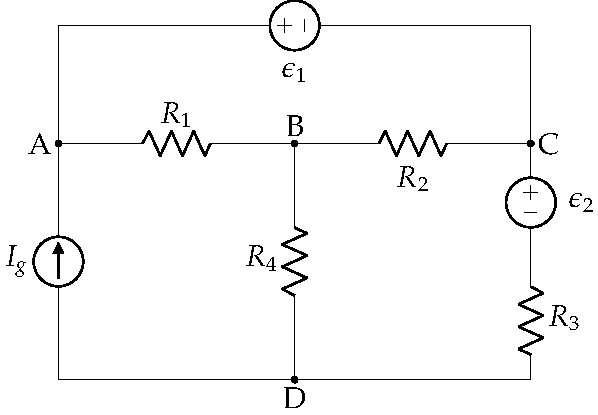
\includegraphics[height=0.5\textheight]{figs/mallas.pdf}
\end{center}
\end{frame}

\begin{frame}[label={sec:org12cff3e}]{Ley de Kirchhoff de las Corrientes (LKC)}
\begin{itemize}
\item La \alert{LKC} es el principio de conservación de la carga aplicado a los circuitos eléctricos.

\item \alert{LKC}: la suma de las corrientes que llegan a un nudo es igual a la suma de las que salen.

\begin{itemize}
\item Las lineas de corriente son cerradas (o solenoidales).
\end{itemize}
\end{itemize}

\begin{center}
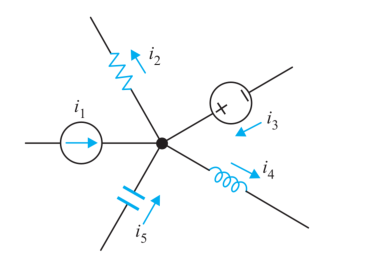
\includegraphics[height=0.4\textheight]{figs/LKC_FM.pdf}
\end{center}
\[
i_1(t) - i_2(t) + i_3(t) - i_4(t) + i_5(t) = 0
\]
\end{frame}

\begin{frame}[label={sec:orgada9c34}]{Ley de Kirchhoff de los Voltajes (LKV)}
\begin{itemize}
\item La \alert{LKV} es el principio de conservación de la energía aplicado a los circuitos eléctricos.

\item \alert{LKV}: la suma (con signo) de las tensiones a lo largo de un camino cerrado (circuito) es cero.

\begin{itemize}
\item La energía producida por un generador es consumida por los receptores del circuito para producir trabajo (mecánico, químico, etc.) o calor.
\end{itemize}
\end{itemize}

\begin{center}
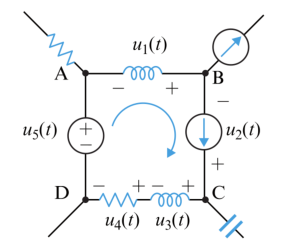
\includegraphics[height=0.4\textheight]{figs/LKV_FM.pdf}
\end{center}
\[
u_3(t) + u_4 (t) - u_5 (t) - u_1 (t) - u_2 (t)  = 0
\]
\end{frame}

\begin{frame}[label={sec:org4ad8f73}]{Balance de Tensiones}
\begin{center}
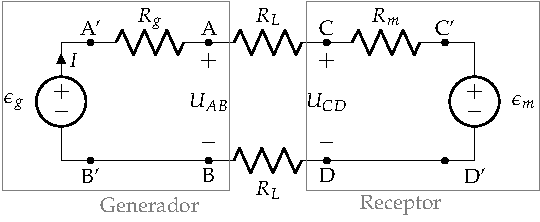
\includegraphics[height=0.5\textheight]{figs/circuito_lkv.pdf}
\end{center}

\begin{equation*}
  U_{A'A} + U_{AC} + U_{CC'} + U_{C'D'} + U_{D'D} + U_{DB} + U_{BB'} + U_{B'A'} = 0
\end{equation*}

\begin{align*}
  U_{AB} &= U_{AA'} + U_{A'B'} + U_{B'B}\\
  U_{CD} &= U_{CC'} + U_{C'D'} + U_{D'D}
\end{align*}
\end{frame}

\begin{frame}[label={sec:org7404429}]{Balance de Tensiones}
\begin{center}
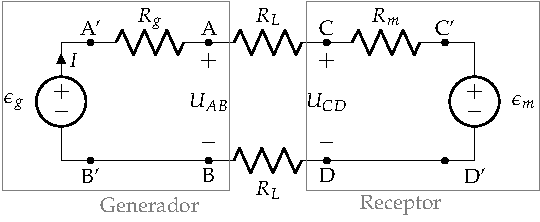
\includegraphics[height=0.25\textheight]{figs/circuito_lkv.pdf}
\end{center}
\begin{equation*}
  U_{A'A} + U_{AC} + U_{CC'} + U_{C'D'} + U_{D'D} + U_{DB} + U_{BB'} + U_{B'A'} = 0
\end{equation*}

\begin{columns}
\begin{column}{0.3\columnwidth}
\begin{align*}
  U_{A'A} &= I \cdot R_g\\
  U_{AC} &= I \cdot R_L\\
  U_{CC'} &= I \cdot R_m\\
  U_{C'D'} &= \epsilon_m\\
  U_{D'D} &= 0 = U_{BB'}\\
  U_{DB} &= I \cdot R_L\\
  U_{B'A'} &= -\epsilon_g
\end{align*}
\end{column}
\begin{column}{0.7\columnwidth}
\begin{equation*}
  \boxed{I \cdot (R_g + 2\cdot R_L + R_m) + \epsilon_m = \epsilon_g}
\end{equation*}
\end{column}
\end{columns}
\end{frame}
\begin{frame}[label={sec:org2834c95}]{Generador y Receptor}
\begin{center}
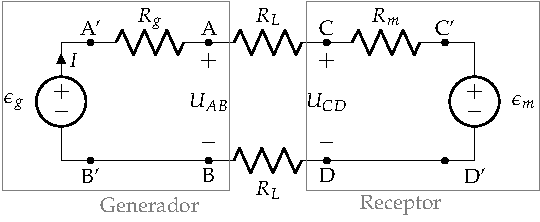
\includegraphics[height=0.25\textheight]{figs/circuito_lkv.pdf}
\end{center}

\begin{columns}
\begin{column}{0.3\columnwidth}
\begin{align*}
  U_{A'A} &= I \cdot R_g\\
  U_{AC} &= I \cdot R_L\\
  U_{CC'} &= I \cdot R_m\\
  U_{C'D'} &= \epsilon_m\\
  U_{D'D} &= 0 = U_{BB'}\\
  U_{DB} &= I \cdot R_L\\
  U_{B'A'} &= -\epsilon_g
\end{align*}
\end{column}
\begin{column}{0.7\columnwidth}
\begin{align*}
  U_{AB} &= U_{AA'} + U_{A'B'} + U_{B'B}\\
  \Aboxed{U_{AB} &= \epsilon_g - I \cdot R_g}
\end{align*}

\begin{align*}
  U_{CD} &= U_{CC'} + U_{C'D'} + U_{D'D}\\
  \Aboxed{U_{CD} &= \epsilon_m + I\cdot R_m}
\end{align*}
\end{column}
\end{columns}
\end{frame}
\subsection{Generadores}
\label{sec:org891feb3}

\begin{frame}[label={sec:orgd1d27cf}]{Ecuación del generador}
Los generadores reales tienen pérdidas que se modelan con una resistencia en \alert{serie} (generador de tensión) o en \alert{paralelo} (generador de corriente)

\begin{columns}
\begin{column}{0.5\columnwidth}
\begin{center}
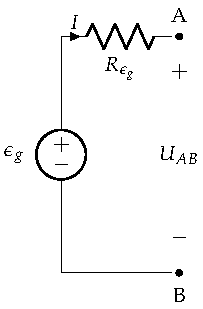
\includegraphics[height=0.5\textheight]{figs/FuenteTensionRealDC.pdf}
\end{center}
\[
  U_{AB} = \epsilon_g - R_{\epsilon_g} \cdot I
\]
\end{column}
\begin{column}{0.5\columnwidth}
\begin{center}
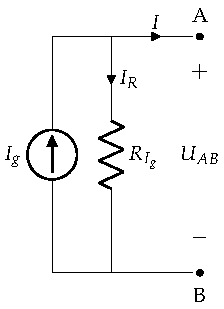
\includegraphics[height=0.5\textheight]{figs/FuenteCorrienteRealDC.pdf}
\end{center}
\[
  I = I_g - \frac{U_{AB}}{R_{I_g}}
\]
\end{column}
\end{columns}
\end{frame}


\begin{frame}[label={sec:org8519c63}]{Equivalencia de Fuentes}
\begin{columns}
\begin{column}{0.25\columnwidth}
\begin{center}
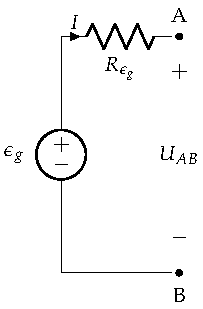
\includegraphics[height=0.45\textheight]{figs/FuenteTensionRealDC.pdf}
\end{center}
\end{column}

\begin{column}{0.5\columnwidth}
\begin{itemize}
\item Dos fuentes son equivalentes cuando suministran el mismo valor de tensión y corriente a un \alert{circuito externo}, para cualquier circuito.

\item Sólo es posible establecer equivalencia entre \alert{fuentes reales}.
\end{itemize}
\end{column}

\begin{column}{0.25\columnwidth}
\begin{center}
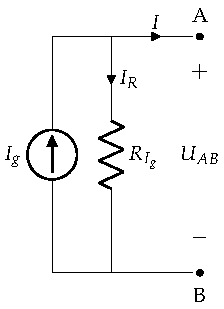
\includegraphics[height=0.45\textheight]{figs/FuenteCorrienteRealDC.pdf}
\end{center}
\end{column}
\end{columns}
\end{frame}


\begin{frame}[label={sec:org19a3910}]{Equivalencia de Fuentes}
\begin{columns}
\begin{column}{0.25\columnwidth}
\begin{center}
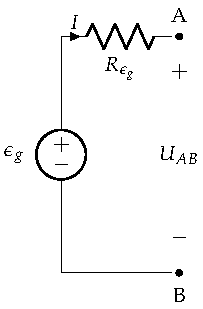
\includegraphics[height=0.43\textheight]{figs/FuenteTensionRealDC.pdf}
\end{center}

\begin{center}
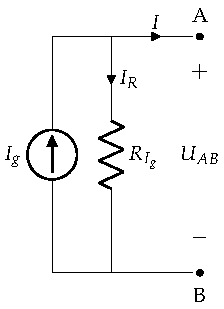
\includegraphics[height=0.43\textheight]{figs/FuenteCorrienteRealDC.pdf}
\end{center}
\end{column}

\begin{column}{0.75\columnwidth}
La salida de tensión de una fuente de tensión es:
\[
  U_{AB} = \epsilon_g - R_{\epsilon_g} \cdot I
\]
Y de una fuente de corriente:
\[
  I = I_g - \frac{U_{AB}}{R_{I_g}} \rightarrow U_{AB} = R_{I_g} \cdot I_g - R_{I_g} \cdot I
\]
Las fuentes son equivalentes cuando las ecuaciones coinciden para cualquier combinación \((U_{AB}, I)\):
\[
\boxed{R_g = R_{\epsilon_g} = R_{I_g}}
\]
\[
  \boxed{\epsilon_g = R_g \cdot I_g} \Leftrightarrow \boxed{I_g = \frac{\epsilon_g}{R_g}}
\]
\end{column}
\end{columns}
\end{frame}

\subsection{Asociación de Elementos}
\label{sec:org0e40ac8}

\begin{frame}[label={sec:org493a6b4}]{Conexión en serie}
\begin{columns}
\begin{column}{0.3\columnwidth}
\begin{center}
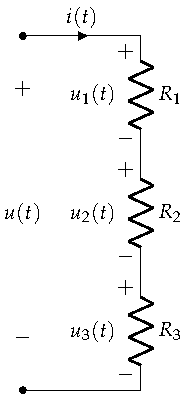
\includegraphics[height=0.85\textheight]{figs/AsociacionSerie.pdf}
\end{center}
\end{column}
\begin{column}{0.7\columnwidth}
Un conjunto de elementos están asociados en serie cuando circula la misma corriente por todos ellos.
\begin{align*}
  u_1(t) &= R_1 \cdot i(t)\\
  u_2(t) &= R_2 \cdot i(t)\\
  u_3(t) &= R_3 \cdot i(t)
\end{align*}
\end{column}
\end{columns}
\end{frame}
\begin{frame}[label={sec:orga47f0e4}]{Conexión en serie}
\begin{columns}
\begin{column}{0.3\columnwidth}
\begin{center}
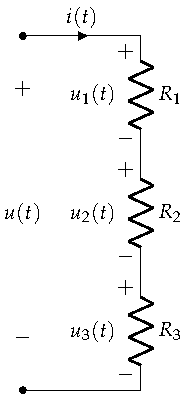
\includegraphics[height=0.85\textheight]{figs/AsociacionSerie.pdf}
\end{center}
\end{column}
\begin{column}{0.7\columnwidth}
Aplicando LKV:
\begin{equation*}
  u(t) = u_1(t) + u_2(t) + u_3(t)
\end{equation*}

Sacando \(i(t)\) como factor común:
\begin{equation*}
  u(t) = i(t) \cdot (R_1 + R_2 + R_3)
\end{equation*}

Definimos la resistencia equivalente de la conexión serie:
\begin{align*}
  \Aboxed{R_s &= \sum_{i = 1}^n R_i}\\
  u(t) &= R_s \cdot i(t)
\end{align*}
\end{column}
\end{columns}
\end{frame}

\begin{frame}[label={sec:org27e3820}]{Divisor de Tensión}
\begin{columns}
\begin{column}{0.3\columnwidth}
\begin{center}
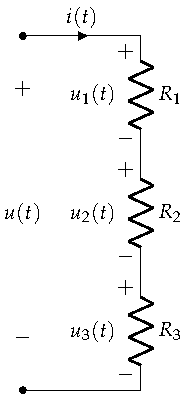
\includegraphics[height=0.85\textheight]{figs/AsociacionSerie.pdf}
\end{center}
\end{column}
\begin{column}{0.7\columnwidth}
De las ecuaciones anteriores tenemos:
\begin{align*}
  i(t) &= \frac{u(t)}{R_1 + R_2 + R_3}\\
  u_3(t) &= R_3 \cdot i(t)\\
\end{align*}

Por tanto, la tensión parcial \(u_3(t)\) se puede expresar en función de la tensión total \(u(t)\): 
\begin{equation*}
  u_3(t) = u(t) \cdot \frac{R_3}{R_1 + R_2 + R_3}  
\end{equation*}

En general:
\begin{equation*}
  \boxed{u_o(t) = u(t) \cdot \frac{R_o}{R_s}}
\end{equation*}
\end{column}
\end{columns}
\end{frame}
\begin{frame}[label={sec:org124b5ad}]{Conexión en serie de inductancias}
\begin{columns}
\begin{column}{0.3\columnwidth}
\begin{center}
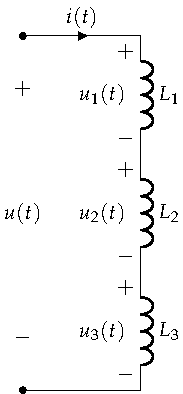
\includegraphics[height=0.85\textheight]{figs/BobinasSerie.pdf}
\end{center}
\end{column}
\begin{column}{0.7\columnwidth}
\begin{align*}
  u_1(t) &= L_1 \cdot \frac{di(t)}{dt}\\
  u_2(t) &= L_2 \cdot \frac{di(t)}{dt}\\
  u_3(t) &= L_3 \cdot \frac{di(t)}{dt}\\
\end{align*}

\begin{align*}
  \Aboxed{L_s &= \sum_{i = 1}^n L_i}\\
  u(t) &= L_s \cdot \frac{di(t)}{dt}
\end{align*}
\end{column}
\end{columns}
\end{frame}

\begin{frame}[label={sec:orgd1a3681}]{Conexión en serie de condensadores}
\begin{columns}
\begin{column}{0.3\columnwidth}
\begin{center}
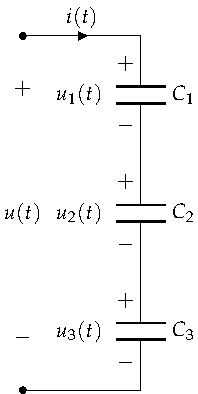
\includegraphics[height=0.85\textheight]{figs/CondensadoresSerie.pdf}
\end{center}
\end{column}
\begin{column}{0.7\columnwidth}
\begin{align*}
  i(t) &= C_1 \cdot \frac{du_1(t)}{dt}\\
  i(t) &= C_2 \cdot \frac{du_2(t)}{dt}\\
  i(t) &= C_3 \cdot \frac{du_3(t)}{dt}\\
\end{align*}

\begin{align*}
  \Aboxed{\frac{1}{C_s} &= \sum_{i = 1}^n \frac{1}{C_i}}\\
  i(t) &= C_s \cdot \frac{du(t)}{dt}
\end{align*}
\end{column}
\end{columns}
\end{frame}

\begin{frame}[label={sec:org4db0957}]{Conexión en paralelo}
Un conjunto de elementos están asociados en paralelo cuando están sometidos a la misma diferencia de potencial.
\begin{center}
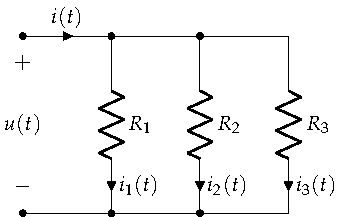
\includegraphics[height=0.45\textheight]{figs/AsociacionParalelo.pdf}
\end{center}

\begin{align*}
  i_1(t) &= u(t)/R_1\\
  i_2(t) &= u(t)/R_2\\
  i_3(t) &= u(t)/R_3
\end{align*}
\end{frame}
\begin{frame}[label={sec:org8dcae46}]{Conexión en paralelo}
\begin{columns}
\begin{column}{0.4\columnwidth}
\begin{center}
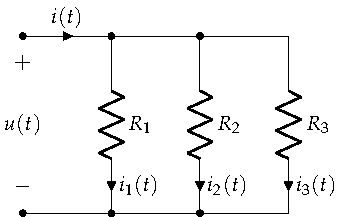
\includegraphics[width=.9\linewidth]{figs/AsociacionParalelo.pdf}
\end{center}
\end{column}
\begin{column}{0.6\columnwidth}
Aplicando LKC:
\begin{equation*}
  i(t) = i_1(t) + i_2(t) + i_3(t)
\end{equation*}

Sacando \(u(t)\) como factor común:
\begin{equation*}
  i(t) = u(t) \cdot (\frac{1}{R_1} + \frac{1}{R_2} + \frac{1}{R_3})
\end{equation*}

Definimos la resistencia equivalente de la conexión paralelo:
\begin{align*}
  \Aboxed{\frac{1}{R_p} &= \sum_{i = 1}^n \frac{1}{R_i}}\\
  u(t) &= R_p \cdot i(t)
\end{align*}
\end{column}
\end{columns}
\end{frame}
\begin{frame}[label={sec:org63aa995}]{Dos resistencias en paralelo}
En el caso concreto de \alert{dos} resistencias en paralelo \ldots{}
\begin{equation*}
  \frac{1}{R_p} = \frac{1}{R_1} + \frac{1}{R_2}
\end{equation*}
\ldots{} la expresión es:
\begin{equation*}
  \boxed{R_p = \frac{R_1 \cdot R_2}{R_1 + R_2}}
\end{equation*}
\end{frame}

\begin{frame}[label={sec:orgaddb53c}]{Conductancia}
Para facilitar las operaciones es conveniente utilizar el inverso de la resistencia:

\begin{equation*}
  G = \frac{1}{R}
\end{equation*}

Así, en lugar de\ldots{}
\begin{align*}
  \frac{1}{R_p} &= \sum_{i = 1}^n \frac{1}{R_i}\\
  u(t) &= R_p \cdot i(t)
\end{align*}

\ldots{} podemos escribir:
\begin{align*}
  \Aboxed{G_p &= \sum_{i = 1}^n G_i}\\
  i(t) &= G_p \cdot u(t)
\end{align*}
\end{frame}

\begin{frame}[label={sec:org033fde3}]{Divisor de corriente}
\begin{columns}
\begin{column}{0.4\columnwidth}
\begin{center}
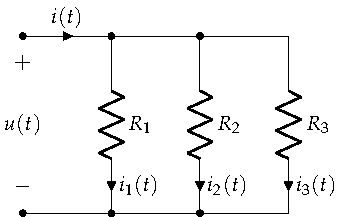
\includegraphics[width=.9\linewidth]{figs/AsociacionParalelo.pdf}
\end{center}
\end{column}
\begin{column}{0.6\columnwidth}
De las ecuaciones anteriores tenemos (usando conductancia):
\begin{align*}
  u(t) &= \frac{i(t)}{G_1 + G_2 + G_3}\\
  i_3(t) &= G_3 \cdot u(t)\\
\end{align*}

Por tanto, la corriente parcial \(i_3(t)\) se puede expresar en función de la corriente total \(i(t)\): 
\begin{equation*}
  i_3(t) = i(t) \cdot \frac{G_3}{G_1 + G_2 + G_3}  
\end{equation*}

En general:
\begin{equation*}
  \boxed{i_o(t) = i(t) \cdot \frac{G_o}{G_p}}
\end{equation*}
\end{column}
\end{columns}
\end{frame}

\begin{frame}[label={sec:org4493eb6}]{Conexión en paralelo de inductancias}
\begin{center}
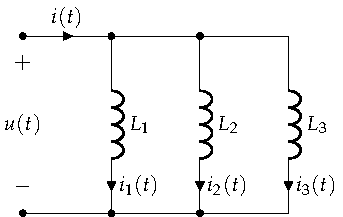
\includegraphics[height=0.45\textheight]{figs/BobinasParalelo.pdf}
\end{center}

\begin{columns}
\begin{column}{0.5\columnwidth}
\begin{align*}
  u(t) &= L_1 \cdot \frac{di_1(t)}{dt}\\
  u(t) &= L_2 \cdot \frac{di_2(t)}{dt}\\
  u(t) &= L_3 \cdot \frac{di_3(t)}{dt}\\
\end{align*}
\end{column}
\begin{column}{0.5\columnwidth}
\begin{align*}
  \Aboxed{\frac{1}{L_p} &= \sum_{i = 1}^n \frac{1}{L_i}}\\
  u(t) &= L_p \cdot \frac{di(t)}{dt}
\end{align*}
\end{column}
\end{columns}
\end{frame}

\begin{frame}[label={sec:org8d794e2}]{Conexión en paralelo de condensadores}
\begin{center}
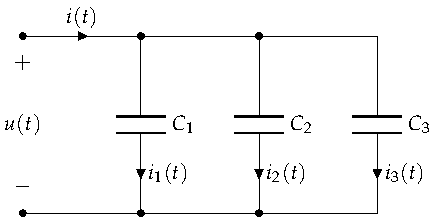
\includegraphics[height=0.45\textheight]{figs/CondensadoresParalelo.pdf}
\end{center}
\begin{columns}
\begin{column}{0.5\columnwidth}
\begin{align*}
  i_1(t) &= C_1 \cdot \frac{du(t)}{dt}\\
  i_2(t) &= C_2 \cdot \frac{du(t)}{dt}\\
  i_3(t) &= C_3 \cdot \frac{du(t)}{dt}\\
\end{align*}
\end{column}
\begin{column}{0.5\columnwidth}
\begin{align*}
  \Aboxed{C_p &= \sum_{i = 1}^n C_i}\\
  i(t) &= C_p \cdot \frac{du(t)}{dt}
\end{align*}
\end{column}
\end{columns}
\end{frame}
\begin{frame}[label={sec:orgd7239d5}]{Conexión Estrella - Triángulo}
\begin{columns}
\begin{column}{0.5\columnwidth}
\begin{center}
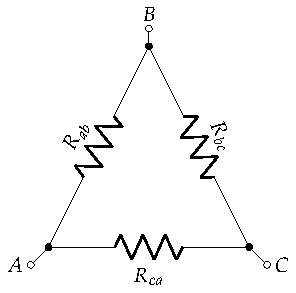
\includegraphics[width=.9\linewidth]{figs/Conexion_Triangulo.pdf}
\end{center}
\end{column}
\begin{column}{0.5\columnwidth}
\begin{center}
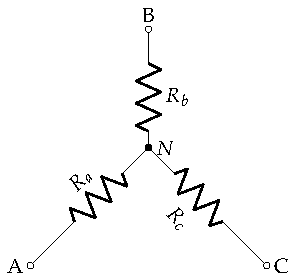
\includegraphics[width=.9\linewidth]{figs/Conexion_Estrella.pdf}
\end{center}
\end{column}
\end{columns}
\end{frame}
\begin{frame}[label={sec:org07cb931}]{Conexión Estrella - Triángulo}
\begin{columns}
\begin{column}{0.5\columnwidth}
\begin{center}
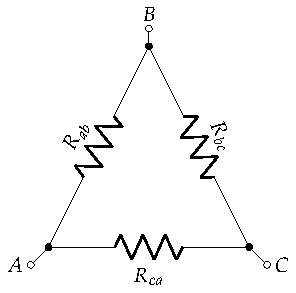
\includegraphics[width=.9\linewidth]{figs/Conexion_Triangulo.pdf}
\end{center}
\end{column}
\begin{column}{0.5\columnwidth}
\begin{align*}
  R_{AB} &= \frac{R_{ab} \cdot (R_{bc} + R_{ca})}{R_{ab} + R_{bc} + R_{ca}}\\
  \\
  R_{BC} &= \frac{R_{bc} \cdot (R_{ab} + R_{ca})}{R_{ab} + R_{bc} + R_{ca}}\\
  \\
  R_{CA} &= \frac{R_{ca} \cdot (R_{ab} + R_{bc})}{R_{ab} + R_{bc} + R_{ca}}
\end{align*}
\end{column}
\end{columns}
\end{frame}
\begin{frame}[label={sec:org2859c8d}]{Conexión Estrella - Triángulo}
\begin{columns}
\begin{column}{0.3\columnwidth}
\begin{center}
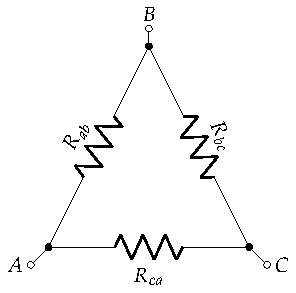
\includegraphics[width=.9\linewidth]{figs/Conexion_Triangulo.pdf}
\end{center}
\end{column}
\begin{column}{0.7\columnwidth}
\begin{align*}
  R_{AB} &= \frac{R_{ab} \cdot R_{bc}}{R_{ab} + R_{bc} + R_{ca}} + \frac{R_{ab} \cdot R_{ca}}{R_{ab} + R_{bc} + R_{ca}}\\
  \\
  R_{BC} &= \frac{R_{bc} \cdot R_{ab}}{R_{ab} + R_{bc} + R_{ca}} + \frac{R_{bc} \cdot R_{ca}}{R_{ab} + R_{bc} + R_{ca}}\\
  \\
  R_{CA} &= \frac{R_{ca} \cdot R_{ab}}{R_{ab} + R_{bc} + R_{ca}} + \frac{R_{ca} \cdot R_{bc}}{R_{ab} + R_{bc} + R_{ca}}
\end{align*}
\end{column}
\end{columns}
\end{frame}
\begin{frame}[label={sec:orgb0b7aa6}]{Conexión Estrella - Triángulo}
\begin{columns}
\begin{column}{0.5\columnwidth}
\begin{center}
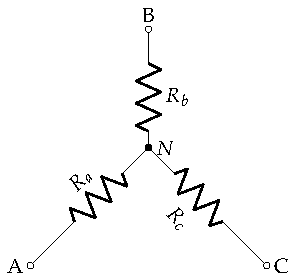
\includegraphics[width=.9\linewidth]{figs/Conexion_Estrella.pdf}
\end{center}
\end{column}
\begin{column}{0.5\columnwidth}
\begin{align*}
  R_{AB} &= R_a + R_b\\
  \\
  R_{BC} &= R_b + R_c\\
  \\
  R_{CA} &= R_c + R_a\\
\end{align*}
\end{column}
\end{columns}
\end{frame}
\begin{frame}[label={sec:orgebf046f}]{Conexión Estrella - Triángulo}
\begin{align*}
  \frac{R_{a{\color{red}b}} \cdot R_{{\color{red}b}c}}{R_{ab} + R_{bc} + R_{ca}} + \frac{R_{{\color{blue}a}b} \cdot R_{c{\color{blue}a}}}{R_{ab} + R_{bc} + R_{ca}} &= R_{\color{blue}a} + R_{\color{red}b}\\
  \\
  \frac{R_{a{\color{red}b}} \cdot R_{{\color{red}b}c}}{R_{ab} + R_{bc} + R_{ca}} + \frac{R_{b{\color{green}c}} \cdot R_{{\color{green}c}a}}{R_{ab} + R_{bc} + R_{ca}} &= R_{\color{red}b} + R_{\color{green}c}\\
  \\
  \frac{R_{{\color{blue}a}b} \cdot R_{c{\color{blue}a}}}{R_{ab} + R_{bc} + R_{ca}} + \frac{R_{b{\color{green}c}} \cdot R_{{\color{green}c}a}}{R_{ab} + R_{bc} + R_{ca}} &= R_{\color{green}c} + R_{\color{blue}a}
\end{align*}
\end{frame}
\begin{frame}[label={sec:orgcbbe7d3}]{Conversión de Triángulo a Estrella}
\begin{columns}
\begin{column}{0.3\columnwidth}
\begin{center}
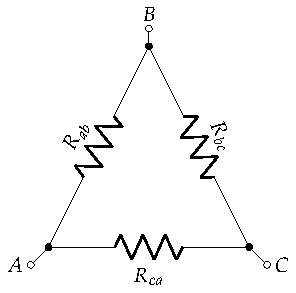
\includegraphics[width=.9\linewidth]{figs/Conexion_Triangulo.pdf}
\end{center}
\end{column}
\begin{column}{0.4\columnwidth}
\begin{align*}
  R_a &= \frac{R_{ab} \cdot R_{ca}}{R_{ab} + R_{bc} + R_{ca}}\\
  \\
  R_b &= \frac{R_{ab} \cdot R_{bc}}{R_{ab} + R_{bc} + R_{ca}}\\
  \\
  R_c &= \frac{R_{bc} \cdot R_{ca}}{R_{ab} + R_{bc} + R_{ca}}
\end{align*}
\end{column}

\begin{column}{0.3\columnwidth}
\begin{center}
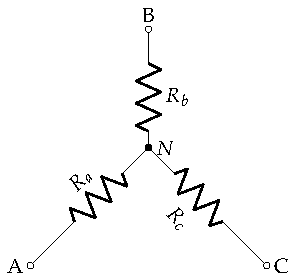
\includegraphics[width=.9\linewidth]{figs/Conexion_Estrella.pdf}
\end{center}
\end{column}
\end{columns}
\end{frame}
\begin{frame}[label={sec:org7a08ca1}]{Conversión de Estrella a Triángulo}
\begin{columns}
\begin{column}{0.3\columnwidth}
\begin{center}
\includegraphics[width=.9\linewidth]{figs/Conexion_Estrella.pdf}
\end{center}
\end{column}
\begin{column}{0.4\columnwidth}
\begin{align*}
  G_{ab} &= \frac{G_a \cdot G_b}{G_a + G_b + G_c}\\
  \\
  G_{bc} &= \frac{G_b \cdot G_c}{G_a + G_b + G_c}\\
  \\
  G_{ca} &= \frac{G_c \cdot G_a}{G_a + G_b + G_c}
\end{align*}
\end{column}
\begin{column}{0.3\columnwidth}
\begin{center}
\includegraphics[width=.9\linewidth]{figs/Conexion_Triangulo.pdf}
\end{center}
\end{column}
\end{columns}
\end{frame}
\section{Métodos de Análisis}
\label{sec:orgb927e17}

\subsection{Método de las mallas}
\label{sec:orgbbfd97e}

\begin{frame}[label={sec:org671bbf0}]{}
\begin{center}
\includegraphics[height=0.95\textheight]{figs/mallas1.pdf}
\end{center}
\end{frame}

\begin{frame}[label={sec:org103946e}]{Aplicamos LKC}
\begin{columns}
\begin{column}{0.5\columnwidth}
\begin{center}
\includegraphics[width=.9\linewidth]{figs/mallas1.pdf}
\end{center}
\end{column}

\begin{column}{0.5\columnwidth}
Nudo A:
\begin{equation*}
  I_6 = I_1 + I_2
\end{equation*}

Nudo B:
\begin{equation*}
  I_1 + I_3 + I_5 = 0
\end{equation*}

Nudo C:
\begin{equation*}
  I_2 = I_3 + I_4
\end{equation*}

Nudo D:
\begin{equation*}
  I_4 = I_5 + I_6
\end{equation*}
\end{column}
\end{columns}

\vspace{5pt}


No son ecuaciones linealmente independientes:
\begin{equation*}
  C = A + B + D
\end{equation*}
\end{frame}

\begin{frame}[label={sec:org290f1b3}]{Aplicamos LKV}
\begin{columns}
\begin{column}{0.5\columnwidth}
\begin{center}
\includegraphics[width=.9\linewidth]{figs/mallas1.pdf}
\end{center}
\end{column}

\begin{column}{0.5\columnwidth}
Malla ABCA
\begin{equation*}
  I_1 \cdot R_1 - \epsilon_1 + \epsilon_2 - I_3 \cdot R_3 - I_2 \cdot R_2 = 0
\end{equation*}

Malla BDCB
\begin{equation*}
  -I_5 \cdot R_5 - I_4 \cdot R_4 + I_3 \cdot R_3 - \epsilon_2 = 0
\end{equation*}

Malla ACDA
\begin{equation*}
  I_2 \cdot R_2 + I_4 \cdot R_4 + I_6 \cdot R_6 - \epsilon_3 = 0
\end{equation*}
\end{column}
\end{columns}
\end{frame}

\begin{frame}[label={sec:orgd4ea940}]{Combinamos las ecuaciones}
\begin{columns}
\begin{column}{0.5\columnwidth}
\begin{center}
\includegraphics[width=.9\linewidth]{figs/mallas1.pdf}
\end{center}
\end{column}

\begin{column}{0.5\columnwidth}
\begin{align*}
  - I_1 -  I_2 + I_6  &= 0\\
  I_1 + I_3 + I_5 &= 0\\
  I_4 - I_5 - I_6 &= 0\\
  I_1 \cdot R_1 - I_2 \cdot R_2 - I_3 \cdot R_3 &= \epsilon_1 - \epsilon_2\\
  I_3 \cdot R_3 - I_4 \cdot R_4 -I_5 \cdot R_5 &= \epsilon_2\\
  I_2 \cdot R_2 + I_4 \cdot R_4 + I_6 \cdot R_6 &= \epsilon_3
\end{align*}
\end{column}
\end{columns}
\end{frame}
\begin{frame}[label={sec:orgc3a0212}]{Y las expresamos en forma matricial}
\begin{equation*}
  \begin{bmatrix}
    -1 & -1 & 0 & 0 & 0 & 1\\
    1 & 0 & 1 & 0 & 1 & 0\\
    0 & 0 & 0 & 1 & -1 & -1\\
    R_1 & -R_2 & - R_3 & 0 & 0 & 0\\
    0 & 0 & R_3 & - R_4 & - R_5 & 0\\
    0 & R_2 & 0 & R_4 & 0 & R_6
  \end{bmatrix} \cdot %
  \begin{bmatrix}
    I_1\\
    I_2\\
    I_3\\
    I_4\\
    I_5\\
    I_6    
  \end{bmatrix} = %
  \begin{bmatrix}
    0\\
    0\\
    0\\
    \epsilon_1 - \epsilon_2\\
    \epsilon_2\\
    \epsilon_3
  \end{bmatrix}
\end{equation*}

Resolver el circuito implica resolver un sistema lineal de 6 ecuaciones, en el que las incógnitas son las corrientes de cada rama.
\end{frame}
\begin{frame}[label={sec:org0cd81bb}]{Método de las mallas}
El método de las mallas simplifica el sistema de ecuaciones necesario mediante unas corrientes \emph{virtuales} denominadas \alert{corrientes de malla}, aprovechando las relaciones entre corrientes de la LKC.

\begin{center}
\includegraphics[height=0.7\textheight]{figs/mallas1_corrientes.pdf}
\end{center}
\end{frame}
\begin{frame}[label={sec:org2cef3b1}]{Relaciones entre las corrientes de rama y malla}
\begin{columns}
\begin{column}{0.6\columnwidth}
\begin{center}
\includegraphics[width=.9\linewidth]{figs/mallas1_corrientes.pdf}
\end{center}
\end{column}
\begin{column}{0.4\columnwidth}
Ramas externas:
\begin{align*}
  I_1 &= I_a\\
  I_5 &= -I_b\\
  I_6 &= I_c
\end{align*}
Ramas internas:
\begin{align*}
  I_2 &= I_c -I_a\\
  I_3 &= I_b - I_a\\
  I_4 &= I_c - I_b
\end{align*}
\end{column}
\end{columns}
\end{frame}
\begin{frame}[label={sec:org5e9a239}]{Ecuaciones de malla}
\begin{center}
\includegraphics[height=0.45\textheight]{figs/mallas1_corrientes.pdf}
\end{center}

Malla ABCA
\begin{equation*}
  I_a \cdot R_1 - \epsilon_1 + \epsilon_2 + (I_a - I_b) \cdot R_3 + (I_a - I_c) \cdot R_2 = 0
\end{equation*}
Malla BDCB
\begin{equation*}
  I_b \cdot R_5 + (I_b - I_c) \cdot R_4 + (I_b - I_a) \cdot R_3 - \epsilon_2 = 0
\end{equation*}
Malla ACDA
\begin{equation*}
  (I_c - I_a) \cdot R_2 + (I_c - I_b) \cdot R_4 + I_c \cdot R_6 - \epsilon_3 = 0
\end{equation*}
\end{frame}
\begin{frame}[label={sec:org619df22}]{Reagrupamos corrientes en las ecuaciones}
\begin{center}
\includegraphics[height=0.5\textheight]{figs/mallas1_corrientes.pdf}
\end{center}

\begin{align*}
  I_a \cdot (R_1 + R_3 + R_2)  - I_b\cdot R_3 - I_c \cdot R_2 &= \epsilon_1 - \epsilon_2\\
  - I_a \cdot R_3 + I_b \cdot (R_5 + R_4 + R_3) - I_c \cdot R_4 &=  \epsilon_2\\
  - I_a \cdot R_2 - I_b \cdot R_4 + I_c \cdot (R_2 + R_4 + R_6) &= \epsilon_3
\end{align*}
\end{frame}
\begin{frame}[label={sec:orga326987}]{Y lo expresamos en forma matricial}
\begin{center}
\includegraphics[height=0.5\textheight]{figs/mallas1_corrientes.pdf}
\end{center}

\begin{equation*}
  \begin{bmatrix}
    (R_1 + R_3 + R_2) &  - R_3 & - R_2 \\
    - R_3 & (R_5 + R_4 + R_3) & - R_4 \\
    - R_2 & - R_4 &  (R_2 + R_4 + R_6)
  \end{bmatrix} \cdot %
  \begin{bmatrix}
    I_a\\
    I_b\\
    I_c\\
  \end{bmatrix} = %
  \begin{bmatrix}
    \epsilon_1 - \epsilon_2\\
    \epsilon_2\\
    \epsilon_3
  \end{bmatrix}
\end{equation*}
\end{frame}
\begin{frame}[label={sec:org4d42ac8}]{Ecuación General}
\begin{equation*}
  \begin{bmatrix}
    {\color{BrickRed}\sum R_{aa}} &  - {\color{MidnightBlue}\sum R_{ab}} & - {\color{MidnightBlue}\sum R_{ca}} \\
    - {\color{MidnightBlue}\sum R_{ab}} & {\color{BrickRed}\sum R_{bb}} & - {\color{MidnightBlue}\sum R_{bc}} \\
    - {\color{MidnightBlue}\sum R_{ca}} & - {\color{MidnightBlue}\sum R_{bc}} &  {\color{BrickRed}\sum R_{cc}}
  \end{bmatrix} \cdot %
  \begin{bmatrix}
    I_a\\
    I_b\\
    I_c\\
  \end{bmatrix} = %
  \begin{bmatrix}
    {\color{OliveGreen}\sum\epsilon_a}\\
    {\color{OliveGreen}\sum\epsilon_b}\\
    {\color{OliveGreen}\sum\epsilon_c}
  \end{bmatrix}
\end{equation*}
\begin{description}
\item[{\({\color{BrickRed}\sum R_{aa}}\)}] suma de las resistencias incluidas en la malla de \(I_a\).
\item[{\({\color{MidnightBlue}\sum R_{ab}}\)}] suma de las resistencias incluidas en las ramas compartidas por las mallas de \(I_a\) e \(I_b\).
\item[{\({\color{OliveGreen}\sum \epsilon_a}\)}] suma algebraica de las fuerzas electromotrices de los generadores de la malla de \(I_a\). Su signo es positivo si contribuyen al giro de la corriente.
\end{description}
\end{frame}
\begin{frame}[label={sec:org6d6f743}]{Procedimiento}
\begin{enumerate}
\item Identificar las corrientes de rama.
\item Asignar un sentido a las corrientes de malla.
\item Relacionar corrientes de rama con corrientes de malla.
\item Escribir ecuación de mallas.
\item Resolver la ecuación, obteniendo las corrientes de malla.
\item Obtener las corrientes de rama con las relaciones del punto 3.
\end{enumerate}

\alert{Importante}: todos los generadores deben ser fuentes de tensión.
\end{frame}

\subsection{Método de los nudos}
\label{sec:orgc423272}
\begin{frame}[label={sec:org675f0c2}]{}
\begin{center}
\includegraphics[width=.9\linewidth]{figs/nudos.pdf}
\end{center}
\end{frame}

\begin{frame}[label={sec:org6e1d306}]{Aplicamos LKC}
\begin{center}
\includegraphics[width=.9\linewidth]{figs/nudos.pdf}
\end{center}

Nudo A
\begin{equation*}
  I_{g1} - I_a - I_{ab} = 0
\end{equation*}

Nudo B
\begin{equation*}
  I_{ab} - I_{g2} - I_b = 0
\end{equation*}
\end{frame}
\begin{frame}[label={sec:org42db2e6}]{Tensiones en las resistencias}
\begin{center}
\includegraphics[width=.9\linewidth]{figs/nudos.pdf}
\end{center}

\begin{align*}
  V_A &= I_a \cdot R_1\\
  V_B &= I_b \cdot R_3\\
  V_{AB} &= I_{ab} \cdot R_2
\end{align*}
\end{frame}
\begin{frame}[label={sec:org6698b50}]{Despejamos las corrientes}
\begin{center}
\includegraphics[width=.9\linewidth]{figs/nudos.pdf}
\end{center}

\begin{align*}
  I_a &= V_A \cdot G_1\\
  I_b &= V_B \cdot G_3\\
  I_{ab} &= (V_A - V_B) \cdot G_2
\end{align*}
\end{frame}


\begin{frame}[label={sec:org038f26d}]{Combinamos las ecuaciones}
\begin{center}
\includegraphics[width=.9\linewidth]{figs/nudos.pdf}
\end{center}

Nudo A
\begin{equation*}
  I_{g1} - V_A \cdot G_1 - (V_A - V_B) \cdot G_2 = 0
\end{equation*}

Nudo B
\begin{equation*}
  (V_A - V_B) \cdot G_2 - I_{g2} - V_B \cdot G_3 = 0
\end{equation*}
\end{frame}


\begin{frame}[label={sec:orgcbc4e6e}]{Reorganizamos las ecuaciones}
\begin{center}
\includegraphics[width=.9\linewidth]{figs/nudos.pdf}
\end{center}

Nudo A
\begin{equation*}
  I_{g1} = V_A \cdot (G_1 + G_2) - V_B \cdot G_2 
\end{equation*}

Nudo B
\begin{equation*}
  - I_{g2} = - V_A \cdot G_2 + V_B \cdot (G_2 + G_3)
\end{equation*}
\end{frame}

\begin{frame}[label={sec:org37b6e34}]{Expresión matricial}
\begin{center}
\includegraphics[width=.9\linewidth]{figs/nudos.pdf}
\end{center}
\begin{equation*}
  \begin{bmatrix}
    G_1 + G_2 & - G_2\\
    -G_2 & G_2 + G_3
  \end{bmatrix} \cdot%
  \begin{bmatrix}
    V_A\\
    V_B
  \end{bmatrix} = %
  \begin{bmatrix}
    I_{g1}\\
    -I_{g2}
  \end{bmatrix}
\end{equation*}
\end{frame}

\begin{frame}[label={sec:org32c595d}]{Ecuación general}
\begin{equation*}
  \begin{bmatrix}
    {\color{BrickRed}\sum G_A} & - {\color{MidnightBlue}\sum G_{AB}} & - {\color{MidnightBlue}\sum G_{AC}}\\
    -{\color{MidnightBlue}\sum G_{AB}} & {\color{BrickRed}\sum G_B} & -{\color{MidnightBlue}\sum G_{BC}}\\
    -{\color{MidnightBlue}\sum G_{AC}} & -{\color{MidnightBlue}\sum G_{BC}} & {\color{BrickRed}\sum G_C}
  \end{bmatrix} \cdot%
  \begin{bmatrix}
    V_A\\
    V_B\\
    V_C
  \end{bmatrix} = %
  \begin{bmatrix}
    {\color{OliveGreen}\sum I_{gA}}\\
    {\color{OliveGreen}\sum I_{gB}}\\
    {\color{OliveGreen}\sum I_{gC}}
  \end{bmatrix}
\end{equation*}

\begin{description}
\item[{\({\color{BrickRed}\sum G_A}\)}] Suma de las conductancias conectadas al nudo \(A\).
\item[{\({\color{MidnightBlue}\sum G_{AB}}\)}] Suma de las conductancias conectadas entre los nudos \(A\) y \(B\).
\item[{\({\color{OliveGreen}\sum I_{gA}}\)}] Suma algebraica de las corrientes de los generadores conectados en el nudo A. El signo es positivo si el generador inyecta corriente en el nudo.
\end{description}

\alert{Importante}: todos los generadores deben ser fuentes de corriente.
\end{frame}
\end{document}